\documentclass[atiam, article]{rapport} % draft, phelma_black, phelma_normal, kit_de, kit_en, phelma_old
\usepackage{booktabs}
\usepackage{float}
\bibliography{truc.bib}

\doctitle{TP Percussions}
\title{TP Percussions\\Accord ou pas d'accord ?}
\titleheader{TP Percussions}
\titleone{}
\titletwo{Acoustique}
\titlethree{}
\author{Paul Estève, Étienne André} % Authors for the header
\autpage{ % Authors for the title page
  \begin{tabular}{l}
    Paul Estève \\
    Étienne André
  \end{tabular}
}
\supervisor[Encadrants : ]{Jean-Loïc Le Carrou\\Christophe Vergez
}
% \supervisorMail{}
\serie{ATIAM 2023/2024}
\date{\today}

\begin{document}

\maketitle

\section{Préparation du TP}

\subsection{Protocole de mesures}
Nous chercherons à mesurer individuellement le comportement de différents instruements après excitation. Nous utiliserons un microphone pour mesurer le champ de pression rayonné. On analysera également en temps réel le son capté avec un spectrogramme et un vu-mètre pour surveiller tout bruit parasite ou saturation.

Afin de disposer d'un éventail de mesures pour chacun des instruments, nous prendrons des mesures de manière uniforme sur sa tessiture, en prenant soin d'inclure les extrêmes. Nous choisirons des points d'excitations représentatifs du jeu d'un percussionniste, et les mailloches typiquement utilisées sur ces instruments.

\begin{itemize}
  \item Vibraphone: point d'excitation au centre de la lame, mailloches de dureté moyenne.
  \item Glockenspiel: point d'excitation au centre de la lame, mailloches dures.
  \item Timbale: point d'excitations du bord jusqu'au centre de la membrane, mailloches souples.
\end{itemize}


Pour le glockenspiel et le vibraphone, le micro sera déplacé pour chaque mesure, dirigé vers le milieu de la lame, à distance fixe.

Pour la timbale, nous envisageons de tester le placement du micro en situation réelle.

\subsection{Reproductibilité de l'excitation}
Afin d'obtenir la même excitation pour toutes les mesures, nous enviseageons de laisser la mailloche pivoter entre nos doigts sous l'effet de la gravité, depuis le même angle et la même position.

\section{Modifications du protocole de mesure}

\subsection{Placement du micro pour la timbale}

Afin de déterminer le meilleur placement de micro, nous avons effectué une mesure préliminaire avec une excitation aux 3/4 du rayon de la membrane. Le micro a été placé successivement
\begin{itemize}
  \item au-dessus centre de la membrane
  \item au-dessus de la moitié du rayon de la membrane, opposé au point de frappe
\end{itemize}

En frappant près du bord de la membrane, la timbale est assimilable à un dipôle rayonnant. On observe donc des annulations dans le spectre lorsque le micro est placé au centre. On placera donc dans la suite le micro dans la seconde position, afin d'éviter ce type de phénomène.

\subsection{Reproductibilité de l'excitation}

Après quelques essais, il s'est avéré que notre méthode d'excitation ne convenait pas:
\begin{itemize}
  \item les frottements entre les doigts et la baguette de la mailloche rendent sa vitesse de chute dépendante du serrage des doigts
  \item il est difficile de garantir un coup unique et n'amortissant pas l'instrument, la mailloche ne rebondissant qu'assez peu
\end{itemize}

Face à ces limitations, nous avons choisi de frapper "à la main". Afin que les excitations soient les plus proches d'un dirac, nous veillons à respecter les mouvements en usage chez les percussionistes, notamment exagérer les mouvements pré- et post-frappe, et utiliser les doigts et le poignet plutôt que les avant-bras.

Pour s'assurer d'une forme de similarité entre toutes les frappes, on surveillera également le niveau de pic maximal grâce à un vu-mètre. Cependant, dans la suite, les amplitudes ne seront pas absolument comparées d'un endroit de la tessiture à l'autre, ainsi une petite disparité d'amplitude est acceptable.

\section{Instruments à lames: Vibraphone et Glockenspiel}
\subsection{Étude théorique}

En modélisant une lame par une poutre libre-libre de matériau isotrope et de section uniforme dans les hypothèses d'Euler-Bernouilli, celle-ci est régie par l'équiation suivante:

$$E I \frac{\partial^4 y}{\partial x^4} + \rho S \frac{\partial^2 y}{\partial t^2} $$
où:
\begin{itemize}
  \item $E$ est le module d'Young du matériau
  \item $I$ est le moment d'inertie
  \item $\rho$ est la densité surfacique de la section
  \item $S$ est la section de la poutre
\end{itemize}

\subsection{Inharmonicité des modes}

On montre que les pulsations modales sont $\omega_n = (\beta_n L)^2 \sqrt{\frac{EI}{\rho L}}$ , où:
\begin{itemize}
  \item $L$ est la longueur de la lame.
  \item $\beta_n$ est solution de $\cos{(\beta_n L)} \cosh{(\beta_n L)} = 1$
\end{itemize}

On a donc la relation $\omega_n = \frac{(\beta_n L)^2}{(\beta_1 L)^2} \omega_1$, dont on calcule numériquement les premières valeurs:
\begin{center}
  \begin{tabular}{ c|c|c|c|c|c|c|c|c } 
    $n$ & 0 & 1 & 2 & 3 & 4 & 5 & 6 & 7 \\
    \hline
    $\beta_n L$ & 0.00 & 4.73 & 7.85 & 11.00 & 14.14 & 17.28 & 20.42 & 23.56 \\
    \hline
    $\frac{\omega_n}{\omega_1}$ & - & 1.00 & 2.76 & 5.40 & 8.93 & 13.34 & 18.64 & 24.81 \\
  \end{tabular}
  \label{table:ratios}
\end{center}

\subsection{Amortissement}

Les lames étant métalliques, les pertes thermo-élastiques sont importantes. Le modèle sans perte ci-dessus peut être adapté en considérant le modèle d'Young complexe et dépendant de $\omega$. On s'attendra donc à observer une décroissance exponentielle de l'amplitude de chaque mode.

\subsection{Traitement des mesures}

Un programme python donné en annexe traite chaque mesure et effectue les opérations suivantes:
\begin{itemize}
  \item Détection du transitoire
  \item Mesure du niveau de bruit de fond avant l'attaque
  \item Réduction du signal à sa partie en oscillation libre (choisi comme étant 0.5s après le transitoire jusqu'au moment où le son atteint le niveau de bruit de fond)
  \item Calcul du spectre
  \item Alignement des fréquences relevées visuellement avec les pics
  \item Calcul des amplitudes et facteurs d'harmonicité des partiels
  \item Tracé des figures et tables incluses dans ce rapport
\end{itemize}

Les partiels étudiés ont été choisis par nos soins visuellement et en basse fréquence afin d'observer clairement les premiers modes. Aucune méthode d'extraction de pics automatique du spectre n'a donné de résultats satisfaisants.

\subsection{Commentaires sur le glockenspiel}

\begin{figure}
  \begin{center}
      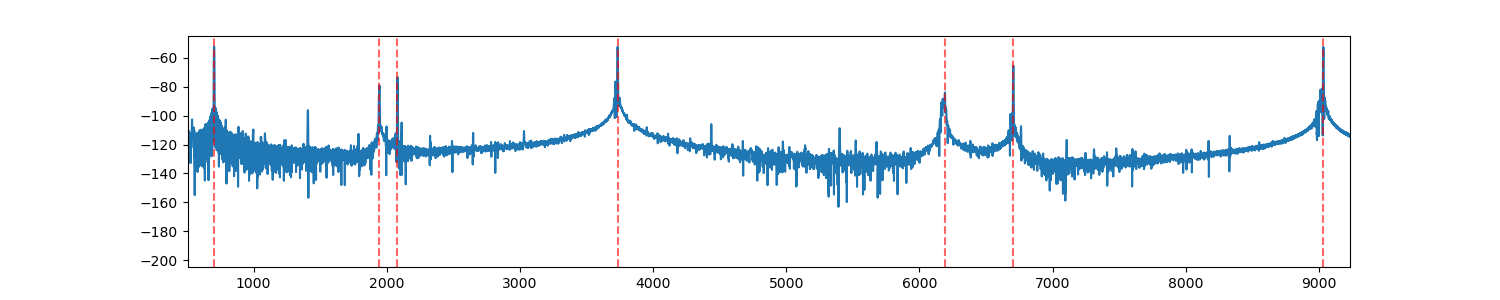
\includegraphics[width=\textwidth]{percu/glock-f5.wav.spectre.png}
  \end{center}
  \caption{Spectre de glock-f5}
  \label{fig:spectre-glock-f5.wav}
\end{figure}
\begin{table}
\centering
\caption{Partiels de glock-f5}
\label{table:partiels-glock-f5.wav}
\begin{tabular}{lrr}
\toprule
{} &  Fréquence (Hz) &  Ratio d'harmonicité \\
\midrule
0 &          703.86 &                 1.00 \\
1 &         1945.13 &                 2.76 \\
2 &         2080.63 &                 2.96 \\
3 &         3737.37 &                 5.31 \\
4 &         6191.16 &                 8.80 \\
5 &         6704.96 &                 9.53 \\
6 &         9033.14 &                12.83 \\
\bottomrule
\end{tabular}
\end{table}


\begin{figure}
  \begin{center}
      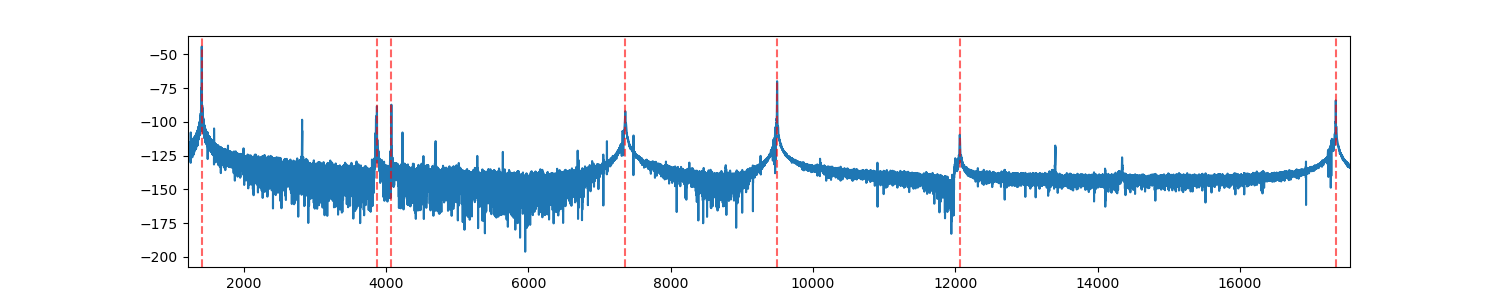
\includegraphics[width=\textwidth]{percu/glock-f6.wav.spectre.png}
  \end{center}
  \caption{Spectre de glock-f6}
  \label{fig:spectre-glock-f6.wav}
\end{figure}
\begin{table}
\centering
\caption{Partiels de glock-f6}
\label{table:partiels-glock-f6.wav}
\begin{tabular}{lrr}
\toprule
{} &  Fréquence (Hz) &  Ratio d'harmonicité \\
\midrule
0 &         1410.64 &                 1.00 \\
1 &         3872.59 &                 2.75 \\
2 &         4075.74 &                 2.89 \\
3 &         7363.04 &                 5.22 \\
4 &         9496.31 &                 6.73 \\
5 &        12063.45 &                 8.55 \\
6 &        17347.69 &                12.30 \\
\bottomrule
\end{tabular}
\end{table}


\begin{figure}
  \begin{center}
      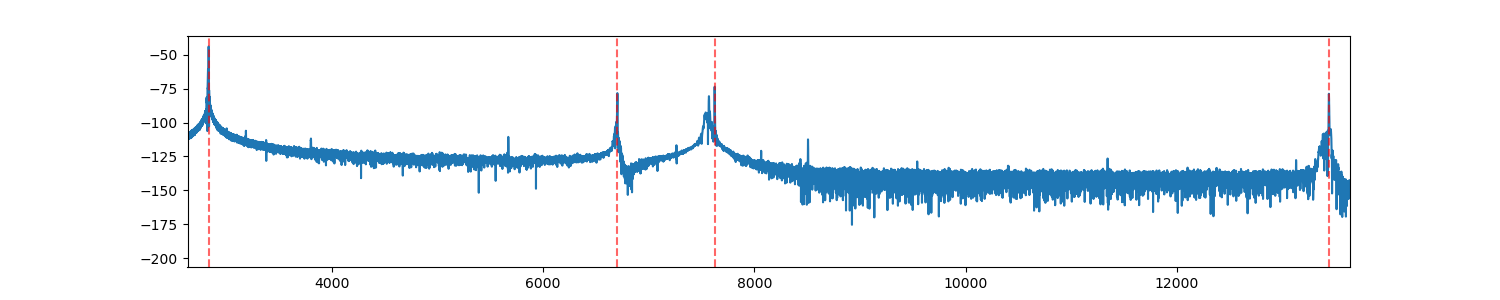
\includegraphics[width=\textwidth]{percu/glock-f7.wav.spectre.png}
  \end{center}
  \caption{Spectre de glock-f7}
  \label{fig:spectre-glock-f7.wav}
\end{figure}
\begin{table}
\centering
\caption{Partiels de glock-f7}
\label{table:partiels-glock-f7.wav}
\begin{tabular}{lrr}
\toprule
{} &  Fréquence (Hz) &  Ratio d'harmonicité \\
\midrule
0 &         2835.94 &                 1.00 \\
1 &         6704.22 &                 2.36 \\
2 &         7624.69 &                 2.69 \\
3 &        13437.56 &                 4.74 \\
\bottomrule
\end{tabular}
\end{table}


On effectue 3 mesures des notes F5 (figure \ref{fig:spectre-glock-f5.wav}, table \ref{table:partiels-glock-f5.wav}), F6 (\ref{fig:spectre-glock-f6.wav}, table \ref{table:partiels-glock-f6.wav}) et F7 (\ref{fig:spectre-glock-f7.wav}, table \ref{table:partiels-glock-f7.wav}); F5 et F7 étant les extrêmes de la tessiture de l'instrument.

On observe les points suivants:
\begin{itemize}
  \item En comparant les ratios avec ceux données dans la table \ref{table:ratios}, on retrouve bien les partiels dont l'inharmonicité est prévue par le modèle théorique.
  \item Selon les notes jouées, d'autres partiels sont également présents. Cela montre les limites du modèle qui prend en compte ni la torsion, ni la traction-compression, et ce dans une seule dimension.
\end{itemize}

\subsection{Commentaires sur le vibraphone}

\begin{figure}
  \begin{center}
      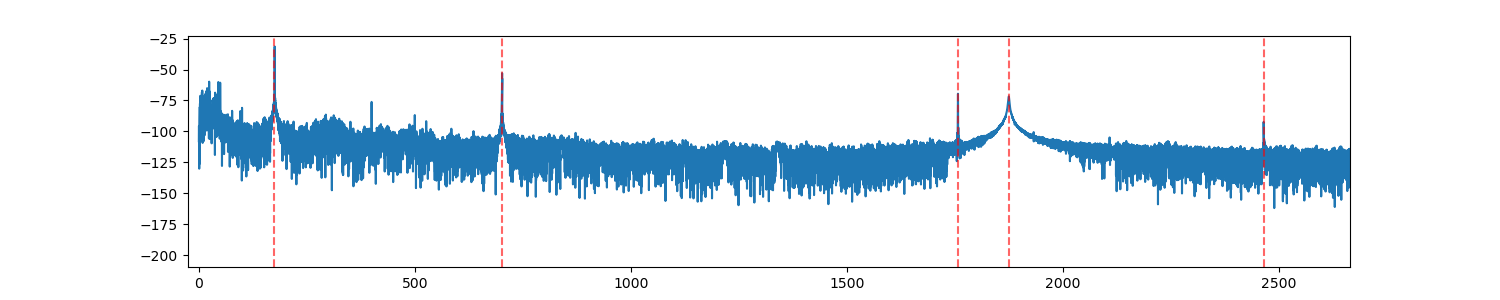
\includegraphics[width=\textwidth]{percu/vibra-f3.wav.spectre.png}
  \end{center}
  \caption{Spectre de vibra-f3}
  \label{fig:spectre-vibra-f3.wav}
\end{figure}
\begin{table}
\centering
\caption{Partiels de vibra-f3}
\label{table:partiels-vibra-f3.wav}
\begin{tabular}{lrr}
\toprule
{} &  Fréquence (Hz) &  Ratio d'harmonicité \\
\midrule
0 &          173.69 &                 1.00 \\
1 &          702.91 &                 4.05 \\
2 &         1757.61 &                10.12 \\
3 &         1875.26 &                10.80 \\
4 &         2465.31 &                14.19 \\
\bottomrule
\end{tabular}
\end{table}


\begin{figure}
  \begin{center}
      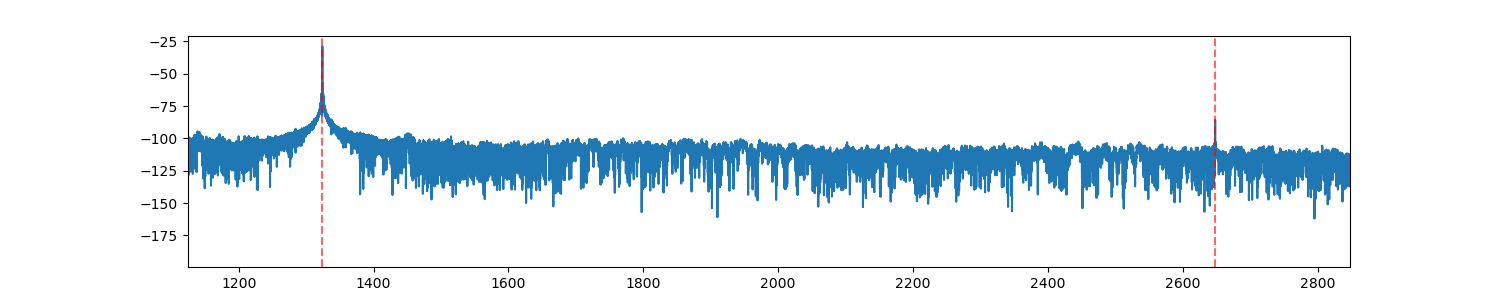
\includegraphics[width=\textwidth]{percu/vibra-e6.wav.spectre.png}
  \end{center}
  \caption{Spectre de vibra-e6}
  \label{fig:spectre-vibra-e6.wav}
\end{figure}
\begin{table}
\centering
\caption{Partiels de vibra-e6}
\label{table:partiels-vibra-e6.wav}
\begin{tabular}{lrr}
\toprule
{} &  Fréquence (Hz) &  Ratio d'harmonicité \\
\midrule
0 &         1324.00 &                 1.00 \\
1 &         2648.00 &                 2.00 \\
\bottomrule
\end{tabular}
\end{table}


On procède de même sur le vibraphone, où on mesure les lames F3 (figure \ref{fig:spectre-vibra-f3.wav}, table \ref{table:partiels-vibra-f3.wav}) et E6 (figure \ref{fig:spectre-vibra-e6.wav}, table \ref{table:partiels-vibra-e6.wav}), les extrêmes de la tessiture de l'instrument. En réalité, la note la plus haute est F6, mais sur l'instrument mis à disposition cette note est amortie par une suspension trop serrée.

Cet instrument se distingue du glockenspiel par ses lames usinées qui ne sont donc plus strictement parallélépipédiques, ce afin notamment d'améliorer leur harmonicité.

Nous mesurons également deux excitations différentes pour A4: au centre (figure \ref{fig:spectre-vibra-a4-centre.wav}, table \ref{table:partiels-vibra-a4-centre.wav}) et au bord (figure \ref{fig:spectre-vibra-a4-bord.wav}, table \ref{table:partiels-vibra-a4-bord.wav}). En effet, lors d'un jeu à 4 baguettes, certains accords sont très difficiles à jouer en frappant au centre des lames sans se contortionner. Le percussionniste préfère alors une position de jeu plus confortable et va frapper certaines lames sur leur bord, afin de garder ses poignets dans la continuité de ses avant-bras.

\begin{figure}
  \begin{center}
      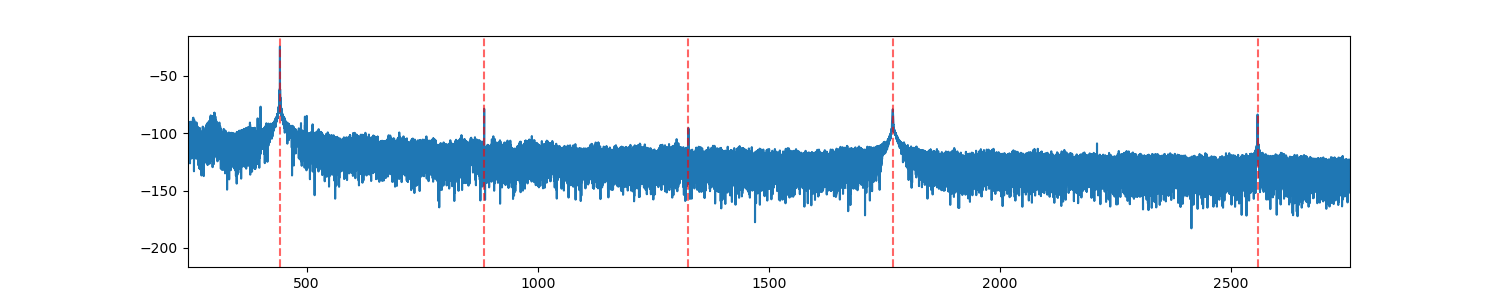
\includegraphics[width=\textwidth]{percu/vibra-a4-bord.wav.spectre.png}
  \end{center}
  \caption{Spectre de vibra-a4-bord}
  \label{fig:spectre-vibra-a4-bord.wav}
\end{figure}
\begin{table}
\centering
\caption{Partiels de vibra-a4-bord}
\label{table:partiels-vibra-a4-bord.wav}
\begin{tabular}{lrr}
\toprule
{} &  Fréquence (Hz) &  Ratio d'harmonicité \\
\midrule
0 &          442.01 &                 1.00 \\
1 &          884.02 &                 2.00 \\
2 &         1326.02 &                 3.00 \\
3 &         1768.08 &                 4.00 \\
4 &         2557.45 &                 5.79 \\
\bottomrule
\end{tabular}
\end{table}


\begin{figure}
  \begin{center}
      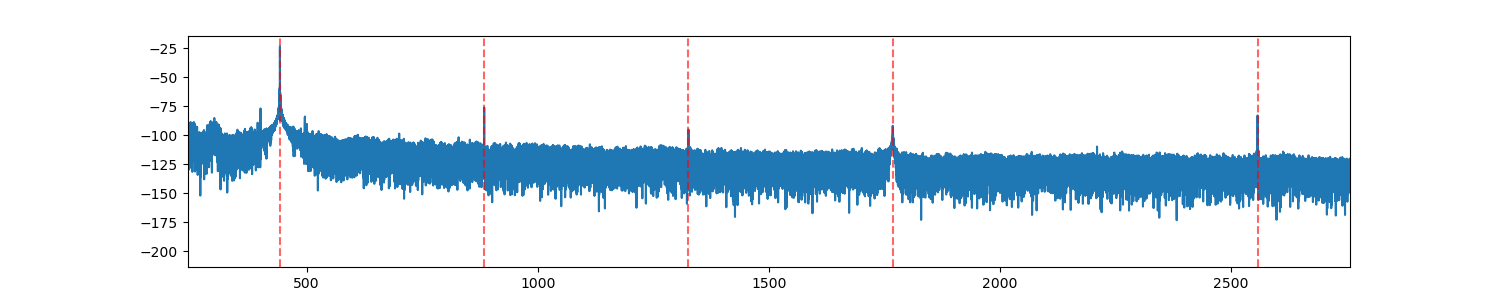
\includegraphics[width=\textwidth]{percu/vibra-a4-centre.wav.spectre.png}
  \end{center}
  \caption{Spectre de vibra-a4-centre}
  \label{fig:spectre-vibra-a4-centre.wav}
\end{figure}
\begin{table}
\centering
\caption{Partiels de vibra-a4-centre}
\label{table:partiels-vibra-a4-centre.wav}
\begin{tabular}{lrr}
\toprule
{} &  Fréquence (Hz) &  Ratio d'harmonicité \\
\midrule
0 &          442.01 &                 1.00 \\
1 &          884.03 &                 2.00 \\
2 &         1326.03 &                 3.00 \\
3 &         1767.95 &                 4.00 \\
4 &         2557.45 &                 5.79 \\
\bottomrule
\end{tabular}
\end{table}


On observe les points suivants:
\begin{itemize}
  \item Frapper au bord ou au centre ne change pas significativement le spectre rayonné.
  \item Une majorité de partiels sont harmoniques, ce qui confère une sensation de hauteur au vibraphone plus marquée que pour le glockenspiel. Cependant, sur F3, on observe une détérioration de l'harmonicité ainsi que plusieurs partiels manquants.
  \item On ne retrouve pas les partiels "parasites" présents sur le glockenspiel, ce qui peut s'expliquer également par l'usinage des lames.
\end{itemize}

\section{Timbale}
\subsection{Étude théorique}

La membrane, supposée fine, parfaitement élastique et de tension uniforme est régie par l'équation:

$$\Delta z(r,\theta, t) = \frac{1}{c^2} \frac{\partial^2 z(r,\theta,t)}{\partial t^2}$$ où:
\begin{itemize}
  \item $z(r,\theta, t)$ est le déplacement de la membrane
  \item $c^2 = \frac{\tau}{\rho}$ avec $\tau$ la tension et $\rho$ la masse surfacique de la membrane
\end{itemize}

Les fréquences modales sont données par $f_{mn} = \frac{j_{mn} c}{2a}$ où
\begin{itemize}
  \item $R$ est le rayon de la membrane
  \item $j_{mn}$ sont les solutions de $J_m(j_{mn}) = 0$, où $J_m$ est la fonction de Bessel de première espèce d'ordre m.
\end{itemize}


\subsection{Comparaison du point d'excitation}

Pour une tension de membrane fixée, on frappe à différents points distribués sur une ligne de rayon de la membrane. On note $a$ la distance du point avec le centre de la membrane et $R$ le rayon de la membrane. On effectue 4 mesures:
\begin{itemize}
  \item $a=3R/4$ (près du bord de la membrane)
  \item $a=R/2$
  \item $a=R/4$
  \item $a=0$ (au centre de la membrane)
\end{itemize}

On obtient les signaux de la figure \ref{fig:timb-position}. On voit (et cela se confirme à l'écoute) que frapper à $a=3R/4$ donne l'amortissement le plus long, et frapper à $a=0$ donne le plus court.

Les spectres sont reproduits dans la figure \ref{fig:timb-position-spectre}. On note qu'aucun des spectres n'est harmoniques, ce qui est attendu. Le spectre pour $a=0$ est particulièrement non-musical. On observe cependant que le spectre des autres points d'excitations sont assez similaires.

On s'intéressera donc dans la suite au point d'excitation $a=3R/4$, ce qui correspond à la technique de jeu orchestrale standard.

\begin{figure}
  \begin{center}
    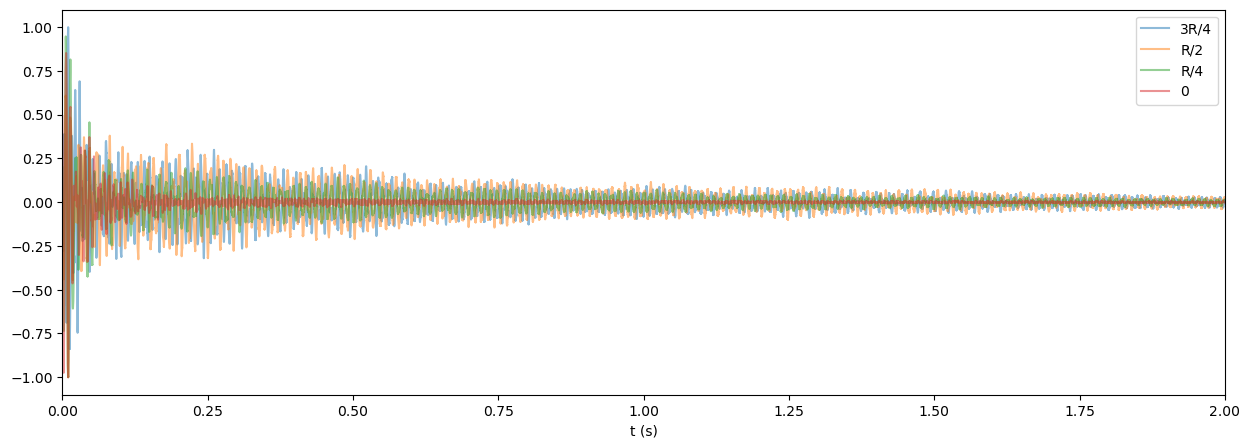
\includegraphics[width=\textwidth]{percu/timbale-position-frappe-temps.png}
  \end{center}
  \caption{Signaux pour différents points d'excitation}
  \label{fig:timb-position}
\end{figure}

\begin{figure}
  \begin{center}
    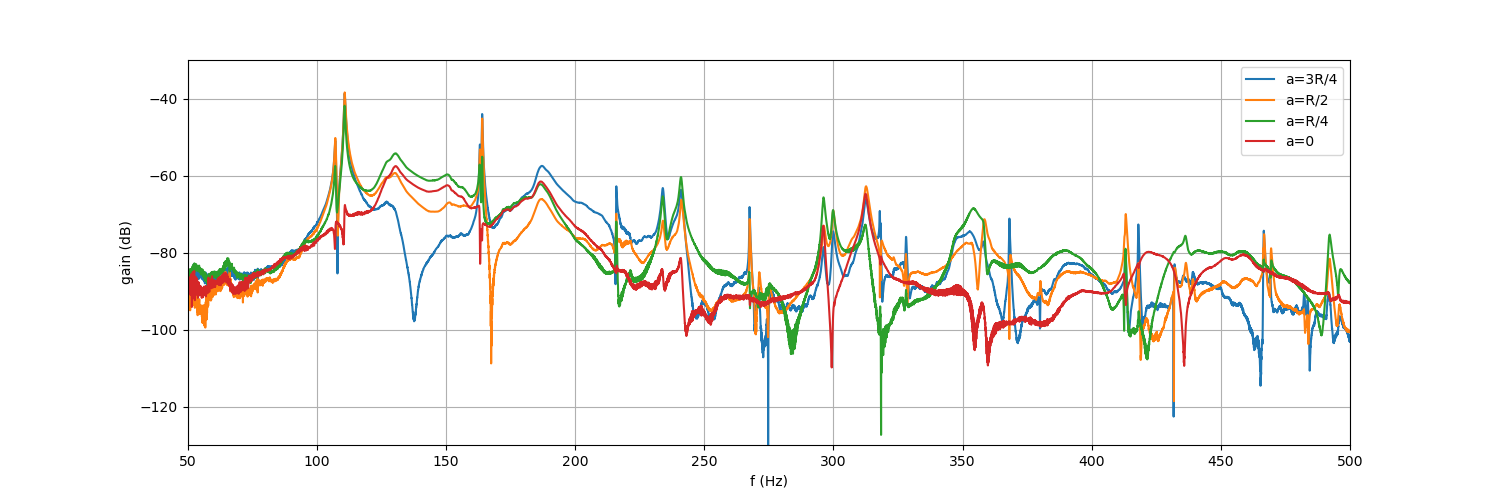
\includegraphics[width=\textwidth]{percu/timbale-position-frappe.png}
  \end{center}
  \caption{Spectres pour différents points d'excitation}
  \label{fig:timb-position-spectre}
\end{figure}

\subsection{Inharmonicité}

On a reproduit les spectres respectifs dans les figures \ref{fig:timb-grave-spectre}, \ref{fig:timb-migrave-spectre} et \ref{fig:timb-aigu-spectre} de mesures à $a=3R/4$ pour différentes tensions de la membrane (resp. minimale, moyenne et maximale) réglée à l'aide de sa pédale de tension. On a ajouté en pointillés noirs les valeurs théoriques des fréquences propres des premiers modes.

On peut noter que les pics du spectre mesuré s'approchent mais ne correspondent pas aux fréquences théoriques: le modèle présenté à la section prédédente ne prend pas en compte ni le rayonnement, ni le couplage avec la cuve.

\begin{figure}
  \begin{center}
    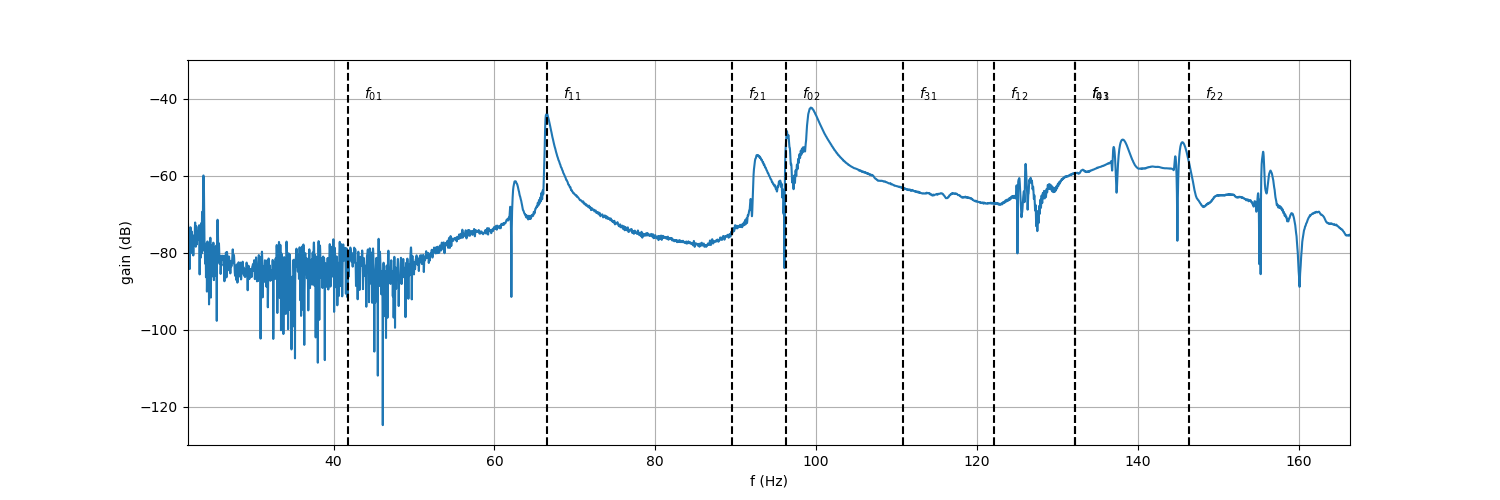
\includegraphics[width=\textwidth]{percu/timbale-grave-spectre.png}
  \end{center}
  \caption{Spectre pour $a=3R/4$, tension minimum}
  \label{fig:timb-grave-spectre}
\end{figure}


\begin{figure}
  \begin{center}
    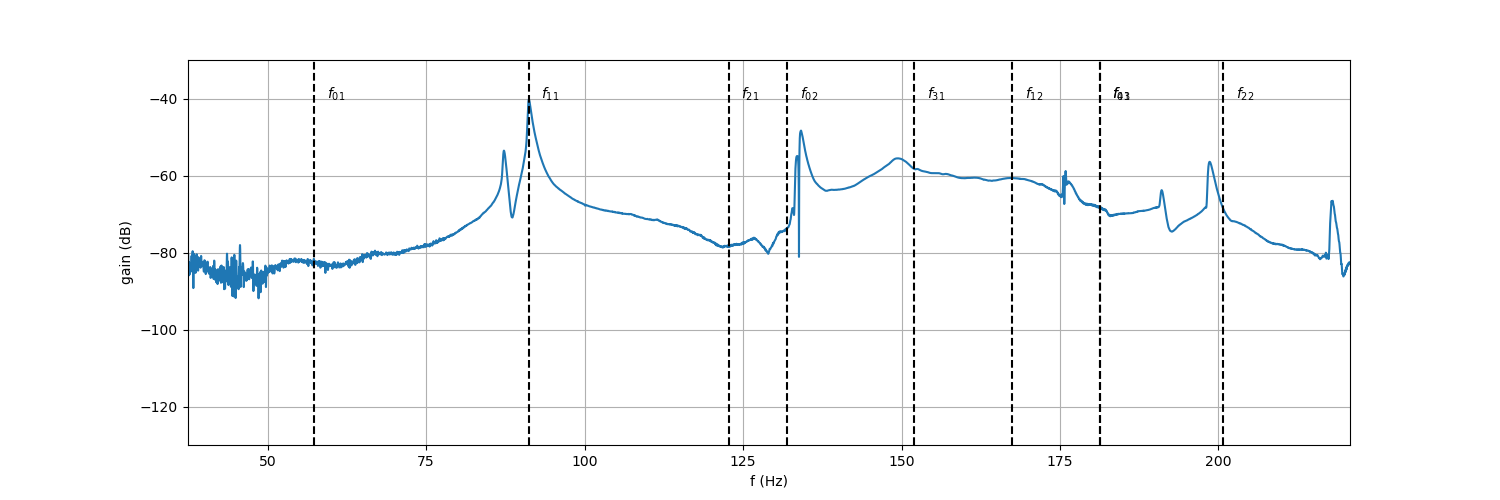
\includegraphics[width=\textwidth]{percu/timbale-migrave-spectre.png}
  \end{center}
  \caption{Spectre pour $a=3R/4$, tension moyenne}
  \label{fig:timb-migrave-spectre}
\end{figure}

\begin{figure}
  \begin{center}
    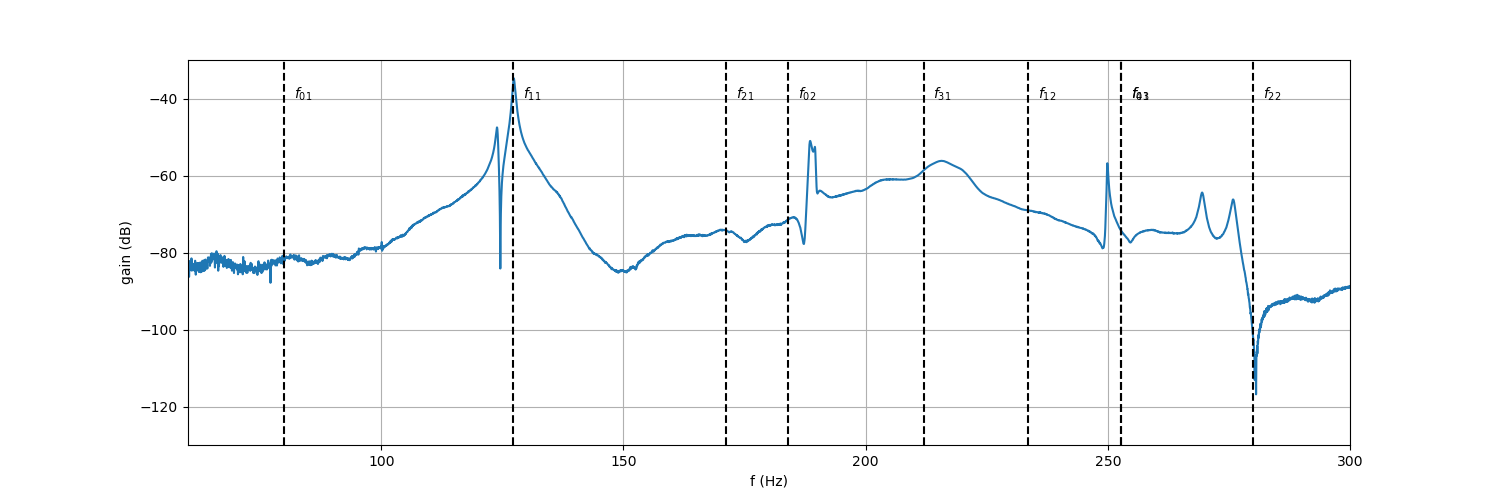
\includegraphics[width=\textwidth]{percu/timbale-aigu-spectre.png}
  \end{center}
  \caption{Spectre pour $a=3R/4$, tension maximum}
  \label{fig:timb-aigu-spectre}
\end{figure}

Pour continuer la comparaison, la figure \ref{fig:comparaison-harmo-timbale} montre les différences d'accord des différents partiels pour plusieurs tensions de la membrane. L'axe des fréquences est ramené à la même échelle afin de permettre la comparaison entre les différentes courbes, et est gradué en octaves et en quintes.

On remarque en premier lieu que les positions des pics ne sont pas strictement égales selon la tension. Toutefois, on observe que pour toutes les tensions, le deuxième partiel est accordé autour de la première quinte, et le deuxième autour de l'octave, ce qui contribue à la sensation de hauteur de note à l'écoute. On observe pour finir que plus la tension augmente, plus les pics s'approchent des harmoniques (et quintes), ce qui est également confirmé à l'écoute.

\begin{figure}
  \begin{center}
    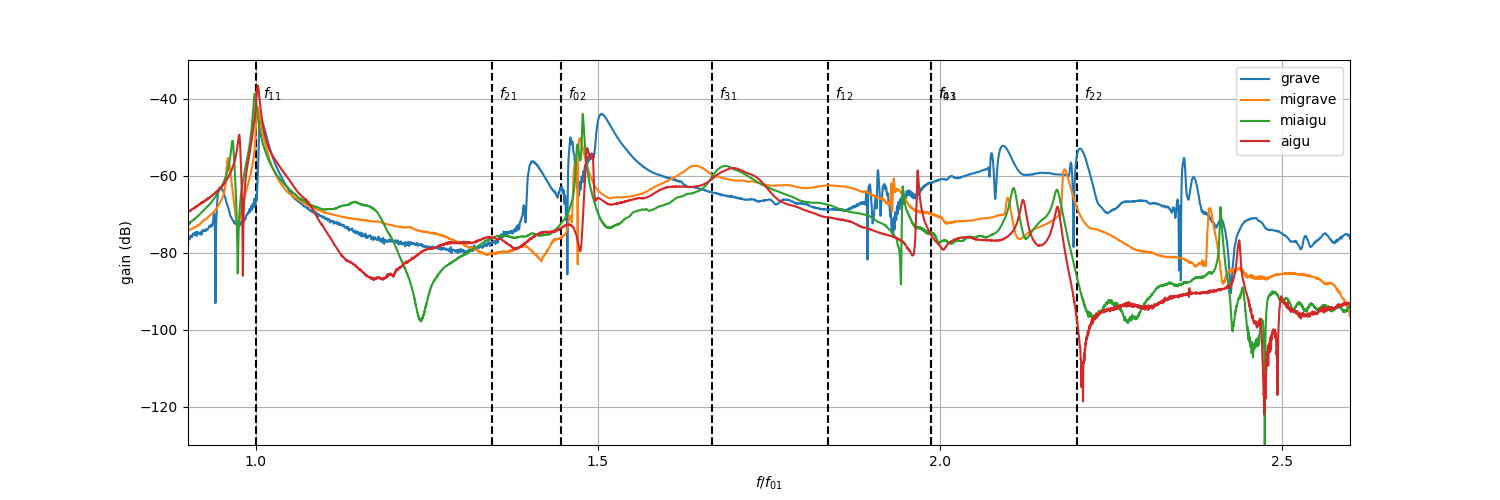
\includegraphics[width=\textwidth]{percu/comparaison-harmo-timbale.png}
  \end{center}
  \caption{Spectres en fréquence ramenée}
  \label{fig:comparaison-harmo-timbale}
\end{figure}

\subsection{Dureté des mailloches}

On s'intéresse enfin à l'influence de la dureté des mailloches sur le son produit. Pour observer ceci, on mesure deux réponses à deux excitations au même point, avec la même tension de membrane, mais avec des mailloches de dureté différentes. Les spectres (smoothés avec un filtre de Savitzky-Golay pour faciliter la lecture) résultants sont reproduits figure \ref{fig:timb-soft-hard}.

On observe que si la forme des deux spectres est très similaire, celui produit par la baguette dure a un contenu plus riche en hautes fréquences. Cela s'explique par la forme de l'excitation, qu'on peut modéliser par une fonction porte dont la largeur diminue avec la dureté des mailloches. Dans le domaine fréquence, celle-ci agit comme un filtre passe-bas dont la fréquence augmente avec la largeur de la porte.

\begin{figure}
  \begin{center}
    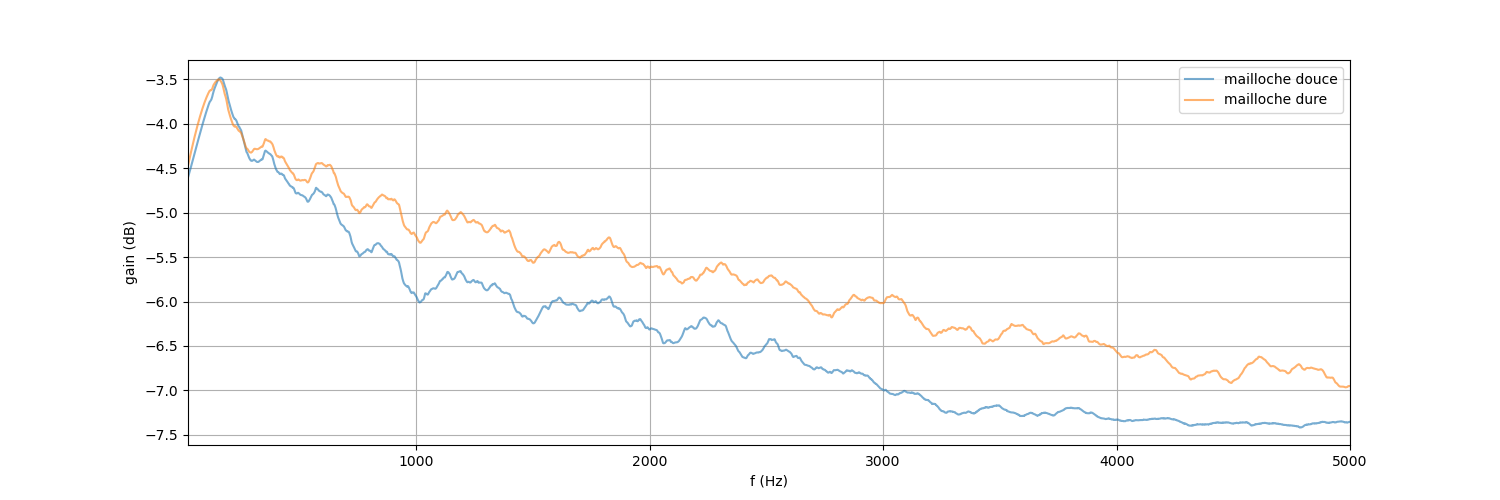
\includegraphics[width=\textwidth]{percu/timbale-soft-hard.png}
  \end{center}
  \caption{Comparaison de mailloches de dureté différente}
  \label{fig:timb-soft-hard}
\end{figure}

\section{Conclusion}

Nous avons mis en évidence l'influence de différents facteurs sur le timbre du glockenspiel, du vibraphone et timbale.

Le facteur d'instrument est garant de l'(in)harmonicité de l'instrument : en choisissant judicieusement le dimensionnement de diverses grandeurs, ou encore en usinant la forme des éléments vibrants comme pour le vibraphone, il peut en ajuster les fréquences propres et donc son timbre.

Mais même si le musicien ne peut pas contrôler les fréquences propres, il est cependant dans son rôle d'être attentif à sa technique de jeu, qui peut alors influer sur les amplitudes.

\printbibliography

\end{document}